\chapter*{Introduzione al corso}
\addcontentsline{toc}{chapter}{Introduzione al corso}

L'obiettivo del corso "Architettura degli elaboratori" è quello di capire da cosa è formato un calcolatore ed il suo funzionamento in relazione alla comunicazione con il codice. Durante il corso, inoltre, conosceremo le strutture delle principali CPU moderne.

In particolar modo gli argomenti del corso saranno:
\begin{itemize}
    \item Introduzione storica e struttura di una CPU;
    \item L'assembler MIPS;
    \item Progetto della CPU MIPS ad un colpo di clock;
    \item Introduzione alla pipeline;
    \item Progetto della CPU MIPS con pipeline;
    \item Gestione degli hazard ed eccezioni;
    \item Gerarchia di memoria e cache;
    \item Parallelismo con cache;
    \item Memoria virtuale e protezione.
\end{itemize}

L'esame sarà diviso in due parti: una prova pratica che riguarda la programmazione assembly e una prova scritta.
\subsubsection{Gerarchia hardware-software}
Una delle prime domande che ci poniamo è come è possibile tradurre da linguaggio di alto livello a linguaggio comprensibile dal calcolatore?

Ebbene come vedremo più avanti, il calcolatore può solo eseguire istruzioni di basso livello estremamente semplici. Per passare da 
un’applicazione complessa (scritta in un linguaggio vicino a quello dell’essere umano) alle semplici istruzioni che possono essere comprese dal calcolatore si utilizza un processo che coinvolge  diversi strati di software. 

\begin{figure}[H]
    \centering
    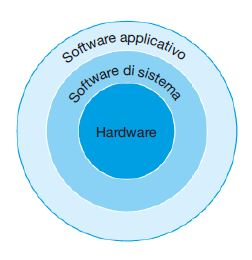
\includegraphics[height=5cm]{images/gerarchia_hardware_software.JPG}
    \caption{Gerarchia hardware-software}
    \label{fig:gerarchia_hardware_software}
\end{figure}
Questi strati sono organizzati principalmente in maniera gerarchica come mostrato in Figura \ref{fig:gerarchia_hardware_software}. Nel cerchio più esterno compaiono le applicazioni, mentre i diversi componenti del software di sistema sono posizionati nel cerchio intermedio, a cui fanno parte il sistema operativo che permette di 
interfacciare i programmi utente con l’hardware del calcolatore e i compilatori che permettono la traduzione di un programma scritto in un linguaggio ad alto livello, in istruzioni eseguibili dall’hardware.

\subsubsection{Architettura del calcolatore}
Architettura dell’insieme di istruzioni (ISA): detta anche semplicemente architettura è un'interfaccia astratta tra l’hardware e il livello più basso del software di un calcolatore. Comprende tutte le informazioni necessarie per scrivere un programma in linguaggio macchina funzionante in modo corretto, comprese le istruzioni, i registri, gli accessi a memoria, l’I/O, l'unità di controllo (indica cosa fare in base alle
istruzioni del programma), l'unità di elaborazione dei dati (effettua operazioni artimetico-logiche) ecc.

\subsubsection{Unità di misura e prestazioni della CPU}
\begin{table}[H]
    \centering
    \begin{tabular}{|l|c|c|l|c|c|c|}
        \hline
         \textbf{Decimale} & \textbf{Abb} & \textbf{Val} & \textbf{Binario} & \textbf{Abb} & \textbf{Val} & \textbf{\%} \\\hline\hline
         Kylobyte & KB & $10^3$ & Kibibyte & KiB & $2^{10}$ & 2\%\\\hline
         Megabyte & MB & $10^6$ & Mebibyte & MiB & $2^{20}$ & 5\%\\\hline
         Gigabyte & GB & $10^9$ & Gibibyte & GiB & $2^{30}$ & 7\%\\\hline
         Terabyte & TB & $10^{12}$ & Tebibyte & TiB & $2^{40}$ & 10\%\\\hline
         Petabyte & PB & $10^{15}$ & Pebibyte & PiB & $2^{50}$ & 13\%\\\hline
         Exabyte & EB & $10^{18}$ & Exbibyte & EiB & $2^{60}$ & 15\%\\\hline
         Zettabyte & ZB & $10^{21}$ & Zebibyte & ZiB & $2^{70}$ & 18\%\\\hline
         Yottabyte & YB & $10^{24}$ & Yobibyte & YiB & $2^{80}$ & 21\%\\\hline
         Ronnabyte & RB & $1000^9$ & Robibyte & RiB & $2^{90}$ & 24\%\\\hline
         Queccabyte & QB & $10^{10}$ & Quebibyte & QiB & $2^{100}$ & 27\%\\\hline
         
    \end{tabular}
    \caption{Tabella delle unità di misura}
    \label{tab:unità_di_misura}
\end{table}

Nella Tabella \ref{tab:unità_di_misura} sono riportate in forma decimale e binaria le unità di misura riferite ai calcolatori. Nell'ultima colonna, in percentuale, viene indicato quanto l'unità di misura binaria è più grande ripetto alla sua corrispondente decimale.

Grazie a queste unità di misura è possibile fare delle stime sul tempo di esecuzione della CPU.

\begin{equation*}
    \text{\textit{Prestazioni}} = \frac{1}{\text{\textit{Tempo di esecuzione}}}
\end{equation*}

Le metriche più elementari (numero di cicli di clock e periodo del clock) sono legate al tempo di CPU tramite una semplice equazione:
\begin{figure}[H]
    \centering
    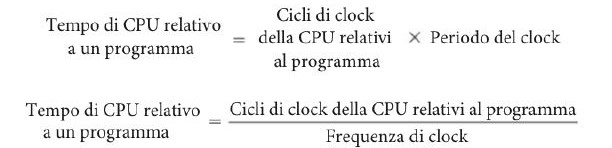
\includegraphics[width=12cm]{images/eq_prestazioni.JPG}
\end{figure}

Un ciclo di clock corrisponde ad un ciclo che partendo dall'elemento di stato, fa se sue operazioni e torna all'inizio. La rappresentazione numerica è basata sui valori di tensione del clock (alto o basso).

\textit{Quanto vale un ciclo di clock?} Come abbiamo visto sopra, dipende dalla frequenza.

Il tempo di esecuzione di un programma non dipende quindi solo dalla frequenza del clock ma anche da:
\begin{enumerate}
    \item Numero di istruzioni di un programma;
    \item CPI (media di clock per istruzione), in quanto ogni istruzione ha un proprio peso;
    \item Frequenza del clock.
\end{enumerate}

\begin{figure}
    \centering
    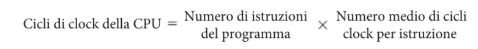
\includegraphics[width=12cm]{images/eq_cicli_clock.JPG}
\end{figure}

\subsubsection{Principi di progettazione}
Con principi di progettazione dell'hardware intendiamo tutte quelle "best practice" che utilizziamo per una migliore resa del prodotto finale:
\begin{enumerate}
    \item La semplicità favorisce la regolarità;
    \item Minori sono le dimensioni, maggiore è la velocità;
    \item Un buon progetto richiede buoni compromessi.
\end{enumerate}